
\chapter{Fixed Target Signal and Backgrounds}

\section{Heavy Photon Production}

Sensitivity to the theoretically favored regions of the heavy photon 
mass-coupling phase space can be best achieved using high luminosity fixed
target experiments \cite{PhysRevD.80.075018}.  In such experiments, an electron
of energy $E_{0}$ incident on a high $Z$ target will radiate heavy photons 
through a process analogous to ordinary photon bremsstrahlung.  The differential
(Fig. \ref{fig:ap_production}).  
\begin{figure}[t]
    \centering
    \caption{A' being produced.}
    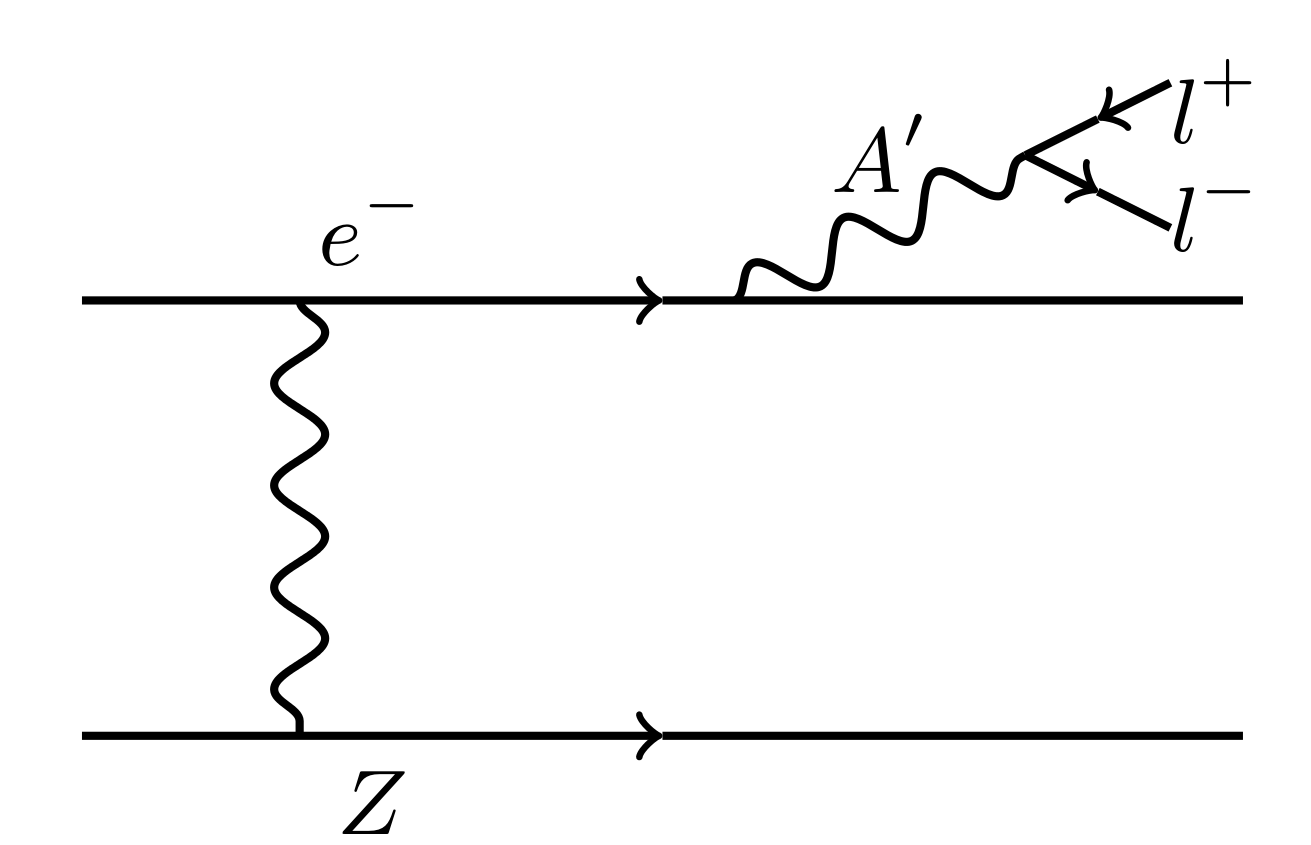
\includegraphics[width=0.5\textwidth]{images/aprime_brem.png}
    \label{fig:ap_production}
\end{figure}  
cross-section of such a process can be estimated using the Weizacker-Williams 
approximation as 
\[
    \frac{\sigma}{dx d\cos{\theta_{A}}} \approx \frac{8 Z^{2} \alpha^{3} \epsilon^{2} E_{0}x}{U^{2}} \chi
            \time [(1 - x + x^{2}/2) - x(1-x)m_{A'}^{2}E_{0}^{2}x\theta_{A'}^{2}/U^{2}]
\]
where $\alpha \sim 1/137$ is the fine structure constant, $\theta_{A}$ is the 
scattering angle of the $A'$, $\chi$ is the effective photon flux and 
\[
    U(x, \theta_{A'}) = E_{0}^{2}x\theta_{A'}^{2} + m_{A'}^{2}\frac{1-x}{x} + m_{e}^2 x
\]
is the virtuality of the intermidiate electron.

%In the case that the mass of the heavy photon is zero, equation
Although heavy photons are produced in a process similar to ordinary bremsstrahlung, 
their production rate and kinematics differ in several ways: 
\begin{itemize}
    \item The production cross-section is suppressed by a factor of $\epsilon^{2}m_{e}^{2}/m_{A'}^{2}$.
    \item The $A'$ is produced very forward.
    \item The $A'$ will take most of the incident beam energy.
\end{itemize}

\section{Trident Backgrounds}

The primary background expected to dominate the final event sample of the Heavy
Photon Search experiment is the quantum electrodynamic Trident process.  As 
shown on Fig. (), the tridents can be seperated out into two main diagrams: 
\begin{figure}[t]
    \centering
    \caption{A' being produced.}
    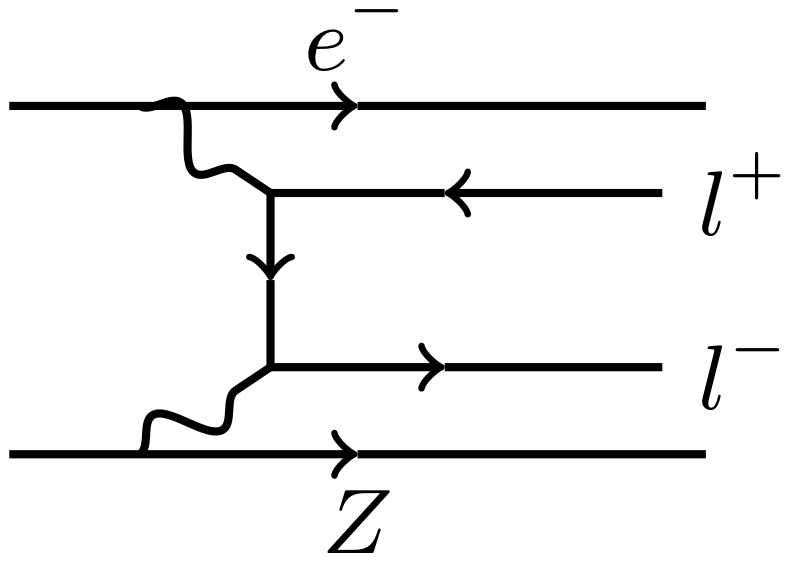
\includegraphics[width=0.5\textwidth]{images/bethe-heitler.png}
    \label{fig:tridents}
\end{figure}  
Bethe-Heitler and radiatives. The kinematics of radiativesare indistinguishable
from the $A'$ signal events within an invariant mass window near the $A'$ mass.
Therefore, radiatives can be used to analyze both the rate of the $A'$ signal 
production and the sensitivity of an experiment to $A'$ signals.  Specifically,
the $A'$ production cross-section is related to the production cross-section of 
radiatives as 
\[
    \frac{d\sigma(A')}{d\sigma(\gamma^*)} = \frac{3\pi\epsilon^{2}}{2 N_{eff} \alpha}
        \frac{m_{A'}}{\delta m}
\]
As a result, the radiatives in the final event sample can be used to analyze 
the $A'$.

Although the rate of the Bethe-Heitler process dominates among the two processes, 
its different kinematics can be used to reduce them in the final event sample.
Specifically, the $A'$ decay products are highly boosted while the recoiling 
electron is soft and scatters at large angles.  In contrast, at higher 
energies, the Bethe-Heitler process is not enhance.  Furthermore, only one of
the leptons in the pair will be highly boosted, while the other will be much
softer.  The recoiling electron will be produced much more forward.


